\chapter{Einleitung}
Dieses Dokument dient der genaueren Beschreibung und Dokumentation des Entwurfs zum Visualisierungstool \gls{programname}, dessen Hauptaufgabe die Darstellung des Netzwerkverkehrs eines \gls{profinet}-Systems ist. Des Weiteren wird der im \gls{ids} \gls{snort} eingebaute \gls{praeprozessor} \gls{sppname} und die genaue Funktionsweise der \gls{ipc} zu \gls{programname} erläutert.\newline
\newline


Das Design von \gls{programname} baut auf dem klassischen \gls{mvc} auf und erweitert diesen Entwurf zu einem \gls{mvp} mit zusätzlicher Funktionalität. Das heisst, dass der Controller aufgeteilt wurde in zwei selbständige Packages. Zum Einen das Service-Package. Dabei handelt es sich um entkoppelte, selbstlaufende Routinen, welche fast die gesamte Logik des Programms ausmachen. Sie werden einmal initialisiert und laufen dann solange \gls{programname} läuft. Zum Andern gibt es den Presenter. Dieser erfüllt seine Hauptaufgabe bei Programmstart. Er instanziiert alle für den Programmablauf benötigten Klassen. Außerdem erstellt er sämtiche nötigen Referenzen, übergibt diese, und startet jeden selbständigen Thread wie zum Beispiel die Services. Danach wird der Presenter nicht mehr benötigt.

Der Entwurf von \gls{programname} baut auf das klassische \gls{mvc} Design auf, welches bereits im Pflichtenheft präsentiert wurde (siehe Abbildung~\ref{fig:old_arch_diagram}). Das erweiterte \gls{mvc} Modell in Abbildung~\ref{fig:arch_diagram} zeigt, dass der Aufbau sich um folgende Bestandteile
\newline\newline
\textbf{MODEL:}\newline
Wie im traditionellen \gls{mvc} Muster dient das Model ausschließlich zur Speicherung von Daten in geeigneten Datenstrukturen. Im Fall von \gls{programname} umfasst dies den Graphen (Kapitel~\ref{subsubsec:graph}), die Programmeinstellungen (Kapitel~\ref{subsubsec:configdata}), ,.
\\
VIEW:
Auch der View unterscheidet sich kaum von der ursprünglichen Funktionalität. Er dient weiterhin dazu, dem Benutzer eine Plattform zur Interaktion mit dem Programm zu bieten. Ein wesentlicher Unterschied zum ursprünglichen Aufbau ist hierbei jedoch, dass der View nur spezifische Interaktionen (siehe INTERACTIONS) kennt und ausführen kann. Wobei der View keine Kenntnis über die hinter der Aktion stehende Logik hat.

INTERACTIONS:
Wie bereits im vorherigen Absatz beschrieben, dienen Interaktionen dem View als 

COMMANDS:
Kommandos sind neben dem SERVICE Package die eigentlichen

PRESENTER:
Im Presenter wird die gesamte Aufbauarbeit geleistet. Kommandos werden mit bestimmten Interaktionen gelinkt, grafische Oberflächen werden instanziiert und vorbereitet und das Modell.
Zusätzlich kümmert sich der Presenter darum, dass sämtliche Service Routinen gestartet werden


Der Presenter ist dafür verantwortlich, dass sämtliche Klassen instanziiert werden

Wie  in


\begin{figure}[H]
  \centering
  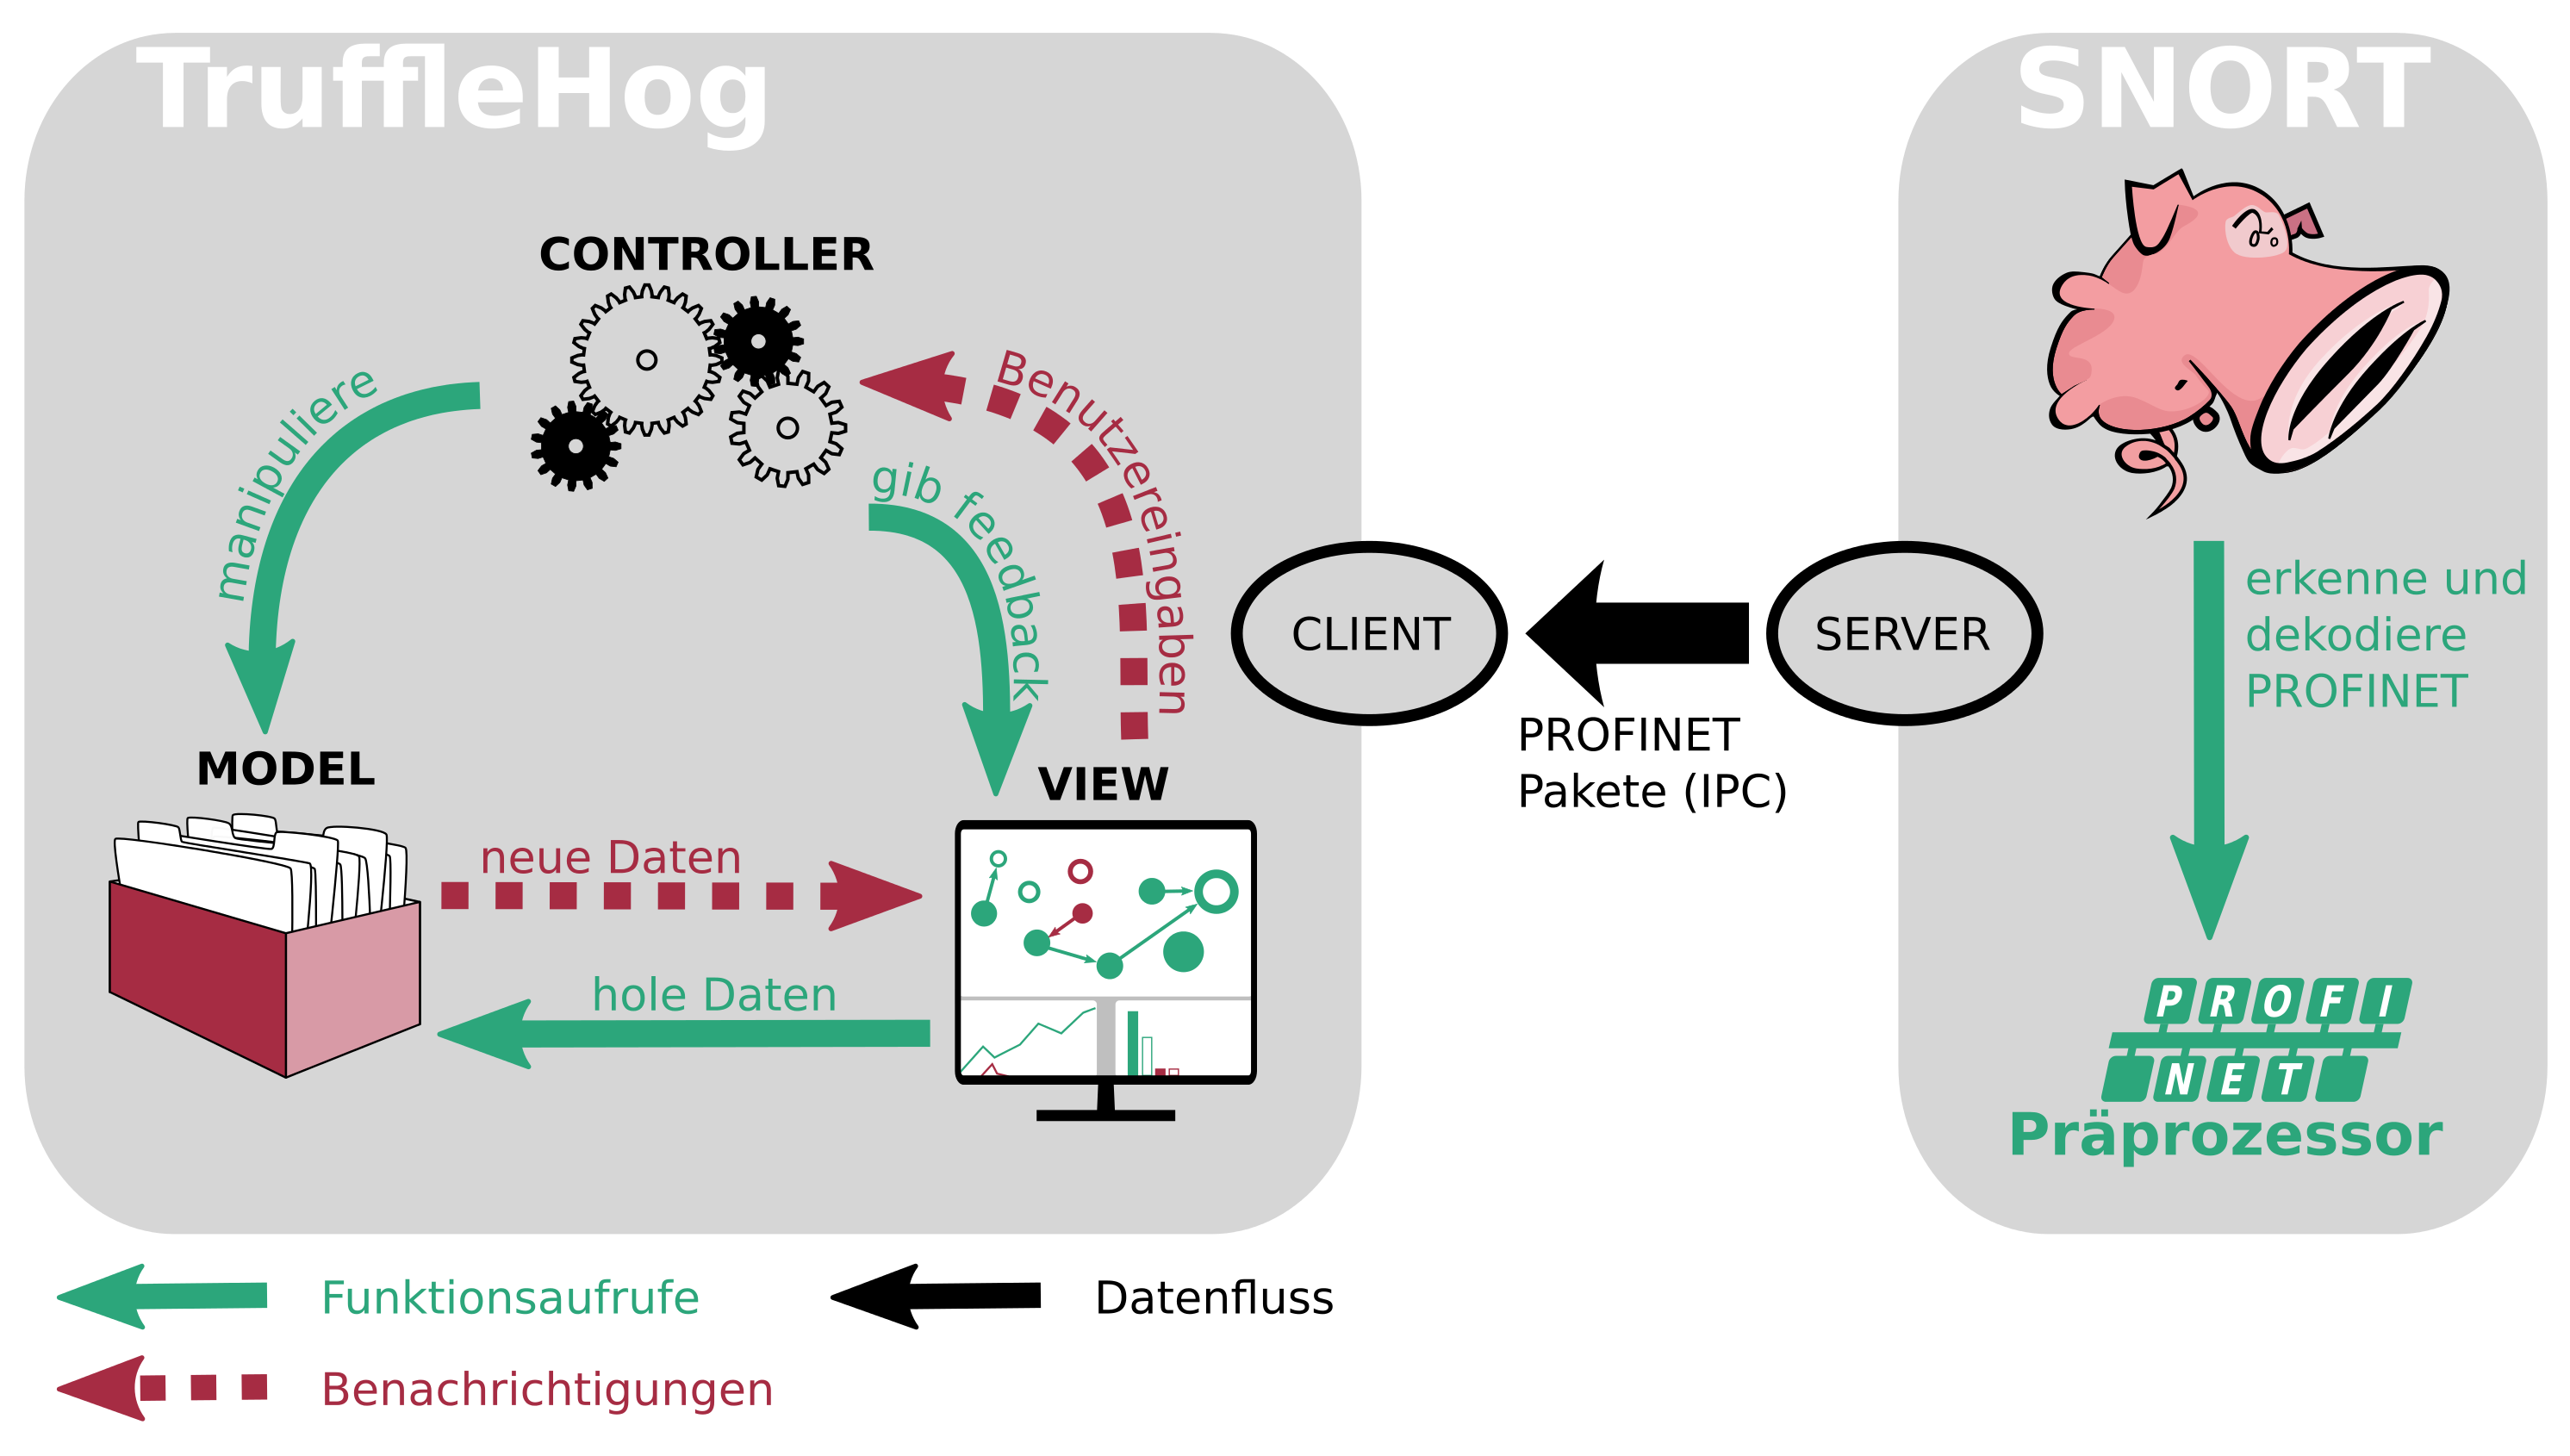
\includegraphics[width=0.8\textwidth]{../diagramimages/praesentationsmodel.png}
  \caption[Ursprüngliche Architektur''ubersicht]{Ursprüngliche Architektur''ubersicht}
  \medskip
  Ursprünglicher Aufbau der Programme aus dem Pflichtenheft
  \label{fig:old_arch_diagram}
\end{figure} 

\begin{figure}[H]
  \centering
  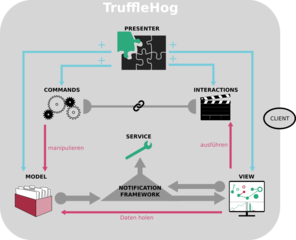
\includegraphics[width=0.8\textwidth]{../diagramimages/arch_diagram_mvp_test.png}
  \caption[Erweiterte Architekturübersicht]{Erweiterte Architekturübersicht}
  \medskip
  Erweiterte Strukturierung des Programms nach dem \gls{mvp} Muster
  \label{fig:arch_diagram}
\end{figure} 
